\chapter{A Segunda Lei da Termodinâmica}
\label{chap:theSecondLaw}

    A nossa experiência cotidiana nos diz que existem tipos de energia que se
    convertem umas nas outras com facilidade, ao passo que o contrário não é
    verdadeiro. Assim, se pisarmos nos freios de um automóvel, a energia
    cinética será transformada em calor e o carro vai eventualmente parar. Mas
    se tiramos o pé do freio, o calor do freio não será reconvertido em energia
    cinética. Da mesma forma, podemos misturar o café ao leite, ao passo que é
    muito complicado e difícil separá-los novamente. Também, por alguma razão o
    calor sempre flui da temperatura mais alta para a temperatura mais baixa e
    nunca ao reverso, bem como o sal flui naturalmente da carne seca para a
    água pura. Mais ainda, afirmamos anteriormente que se deixarmos um sistema
    isolado em paz, ele poderá evoluir espontaneamente para um estado de
    equilíbrio (que depende de suas restrições internas) a partir do qual não
    sairá jamais. Vimos também que utilizando um processo cíclico, não seremos
    capazes de converter todo o calor proveniente de um reservatório térmico em
    trabalho mecânico e, de fato, existe um calor mínimo que deve ser rejeitado
    para o meio-ambiente. O que está por trás de todos estes fenômenos?

    Se lançarmos mão da Primeira Lei, verificaremos com inquietação que, do
    ponto de vista desta, não haveria impedimento algum para que todos estes
    processos impossíveis pudessem ocorrer! De fato, a única pergunta que a
    primeira lei faz ao sistema é a seguinte: \enquote{Energia em todas as suas
    manifestações está se conservando?} Se a resposta for afirmativa, então a
    conclusão seria \enquote{tudo pode}. Precisamos, portanto, de algo mais do
    que a Primeira Lei para se modelar o comportamento da natureza.

    Vamos, então, com auxílio da
    \cref{fig:thermodynamicProcessesSecondLawChapter}, retomar ao nosso
    diagrama de grafos, que muito nos auxiliou para a descoberta da Primeira
    Lei.

    Por hipótese, os processos infinitesimais A, B e C são reversíveis, isto é,
    podem ser exatamente revertidos sem deixar marcas no meio-ambiente ao passo
    que o processo infinitesimal D é irreversível, tendo sido representado em
    linhas pontilhadas, pois sequer conseguimos determinar os seus estados
    intermediários. Lembre-se ainda que todos estes diferentes processos
    ocorrem entre os mesmos estados 1 e 2, que estão, é claro,
    infinitesimalmente à parte.

    \begin{figure}[!htb]
        \caption{%
            Grafo de processos salientando cada \idiff{\gls{heatTransfer}}.
        }

        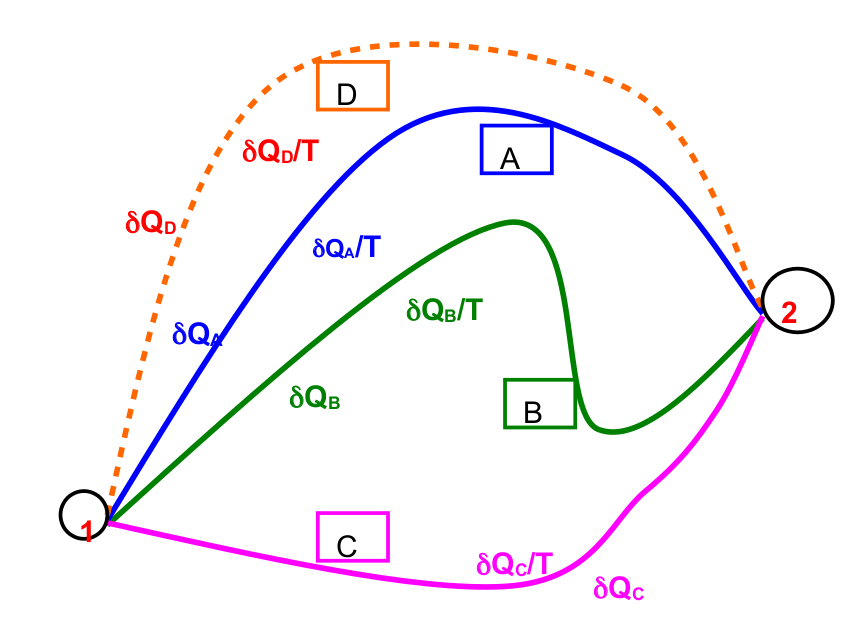
\includegraphics[
            width=0.45\textwidth
        ]   {thermodynamicProcessesSecondLaw.tex}

        \label{fig:thermodynamicProcessesSecondLawChapter}
    \end{figure}

    Já sabíamos que $\idiff{\gls{heatTransfer}_{A}} \neq
    \idiff{\gls{heatTransfer}_{B}} \neq \idiff{\gls{heatTransfer}_{C}} \neq
    \idiff{\gls{heatTransfer}_{D}}$, pois calor, assim como trabalho, é uma
    função de cada processo. Porém se observarmos o comportamento de
    $\dfrac{\idiff{\gls{heatTransfer}}}{\gls{temperature}}$ , onde
    \gls{temperature} é a temperatura que pode variar ao longo do processo,
    para cada processo reversível A, B e C, obteremos o seguinte resultado, que
    até certo ponto é surpreendente:
    %
    \begin{equation} \label{eq:3.1}
        \frac{
            \idiff{\gls{heatTransfer}}
        }{
            \gls{temperature}
        }\bigg)_A^{\gls{reversible}}
        =
        \frac{
            \idiff{\gls{heatTransfer}}
        }{
            \gls{temperature}
        }\bigg)_B^{\gls{reversible}}
        =
        \frac{
            \idiff{\gls{heatTransfer}}
        }{
            \gls{temperature}
        }\bigg)_C^{\gls{reversible}}\,,
    \end{equation}
    %
    isto é, embora os \idiff{\gls{heatTransfer}} sejam todos distintos, os
    $\frac{\idiff{\gls{heatTransfer}}}{\gls{temperature}}$  são idênticos,
    independentemente do processo reversível que consideremos. A propósito,
    $\frac{1}{T}$ é conhecido matematicamente como fator integrante devido ao
    seu papel de transformar uma diferencial inexata em uma diferencial
    ordinária (ou exata).


    \section{A Entropia}

    Da mesma forma que fizemos com a energia total, vamos então definir a
    variação da propriedade termodinâmica entropia como sendo
    %
    \begin{equation} \label{eq:3.2}
        \diff{\gls{entropy}}
        \equiv
        \frac{
            \idiff{\gls{heatTransfer}}
        }{
            \gls{temperature}
        }\bigg)^{\gls{reversible}}\,,
    \end{equation}
    %
    para qualquer processo reversível infinitesimal que vá de 1 até 2.

    Mas o que acontece com o processo irreversível D? Descobriremos que
    %
    %
    \begin{equation} \label{eq:3.3}
        \frac{
            \idiff{\gls{heatTransfer}}
        }{
            \gls{temperature}
        }\bigg)_A^{\gls{reversible}}
        =
        \frac{
            \idiff{\gls{heatTransfer}}
        }{
            \gls{temperature}
        }\bigg)_B^{\gls{reversible}}
        =
        \frac{
            \idiff{\gls{heatTransfer}}
        }{
            \gls{temperature}
        }\bigg)_C^{\gls{reversible}}
        =
        \diff{\gls{entropy}}
        >
        \frac{
            \idiff{\gls{heatTransfer}}
        }{
            \gls{temperature}
        }\bigg)_D^{\gls{irreversible}}\,,
    \end{equation}
    %
    ou seja, para todos os processos irreversíveis, a variação de entropia, que
    só depende dos estados 1 e 2, será sempre maior do que o valor de
    $\dfrac{\idiff{\gls{heatTransfer}}}{\gls{temperature}}$ avaliado ao longo
    daquele processo.

    Resumindo, para qualquer processo especificado em sistemas fechados
    escrevemos a Segunda Lei como:
    %
    \begin{equation}
        \diff{\gls{entropy}}
        \ge
        \underset{j \neq \gls{environmentState}}{\sum }{
            \frac{
                \idiff{\gls{heatTransfer}_{j}}
            }{
                \state{\gls{temperature}}{j}
            }
        }
        +
        \frac{
            \idiff{\gsub{heatTransfer}{environmentState}}
        }{
            \gsub{temperature}{environmentState}
        }\,,
    \end{equation}
    %
    sendo que a igualdade só existirá exclusivamente para processos
    reversíveis.

    Uma formulação muito útil e importante busca eliminar a desigualdade,
    acrescentando-se um termo positivo ou nulo $\mathit{\delta
    S}_{\mathit{gen}}$, que é conhecido como a entropia produzida devido à
    irreversibilidade do processo (você acha que $\mathit{\delta
    S}_{\mathit{gen}}$  é uma propriedade termodinâmica?):
    %
    \begin{equation} \label{eq:3.4}
        \diff{\gls{entropy}}
        =
        \underset{j \neq \gls{environmentState}}{\sum }{
            \frac{
                \idiff{\gls{heatTransfer}_{j}}
            }{
                \state{\gls{temperature}}{j}
            }
        }
        +
        \frac{
            \idiff{\gsub{heatTransfer}{environmentState}}
        }{
            \gsub{temperature}{environmentState}
        }
        +
        \idiff{\gls{entropyCreated}}
        \,\,\,\,
        \text{tal que}
        \,\,\,\,
        \idiff{\gls{entropyCreated}} \ge 0\,.
    \end{equation}

    Na forma integrada, a segunda lei para sistema fechado fica:
    %
    \begin{equation}
        \Delta \gls{entropy}
        =
        \state{\gls{entropy}}{2}
        -
        \state{\gls{entropy}}{1}
        =
        \underset{j \neq \gls{environmentState}}{\sum }{
            \int\limits_1^2
            \frac{
                \idiff{\gls{heatTransfer}_{j}}
            }{
                \state{\gls{temperature}}{j}
            }\bigg)_A
        }
        +
        \frac{
            \fprocess{heatTransfer}{1}{2}{\gls{environmentState}}
        }{
            \gsub{temperature}{environmentState}
        }
        +
        \fprocess{entropyCreated}{1}{2}{A}\,,
    \end{equation}
    %
    com
    %
    \begin{equation} \label{eq:3.5}
        \fprocess{entropyCreated}{1}{2}{A}
        \ge
        0\,.
    \end{equation}

    Note que a integração só poderá ser realizada quando conhecermos a evolução
    de \idiff{\gls{heatTransfer}_{j}} e de \state{\gls{temperature}}{j} ao longo
    de um processo especificado $A$ entre 1 e 2.

    Um enunciado alternativo para a segunda lei afirma que a entropia produzida
    irreversivelmente devido aos processos que ocorrem nos sistemas
    \idiff{\gls{entropyCreated}} é sempre positiva ou no mínimo será nula,
    sendo que este último caso ocorrerá exclusivamente para processos
    reversíveis. Tenha bastante cuidado com a confusão comum entre a entropia
    produzida irreversivelmente \fprocess{entropyCreated}{1}{2}{}, e a variação
    da entropia do sistema $\Delta \gls{entropy}= \state{\gls{entropy}}{2} -
    \state{\gls{entropy}}{1}$ que pode ser positiva, negativa, ou nula.

    Observe também que o trabalho mecânico não desempenha papel algum na
    Segunda Lei da Termodinâmica. Lembra-se quando chamamos a sua atenção para
    a circularidade aparente das definições das energias de calor e de trabalho
    mecânico na fronteira do sistema? Agora já podemos distinguir as duas
    interações de energia entre si sem a necessidade de recorrermos à pressão
    ou à temperatura. Graças à Segunda Lei, sabemos que o calor é aquela
    interação de energia que transporta entropia pela fronteira, ao passo que o
    trabalho mecânico não faz isso. Assim, a entrada de calor em um sistema
    implica aumento da entropia do sistema e vice-versa para a saída de calor
    do sistema.


    \section{Consequências da Segunda Lei para Sistema Fechado}

    Seja um processo adiabático ocorrendo em um sistema fechado. Aplicando-se a
    Segunda Lei ao sistema, ficamos com
    %
    \begin{equation} \label{eq:3.6}
        \Delta\gls{entropy}
        =
        \state{\gls{entropy}}{2}
        -
        \state{\gls{entropy}}{1}
        =
        \fprocess{entropyCreated}{1}{2}{A}
        \ge 0
    \end{equation}
    %
    ou seja, sob qualquer processo adiabático em um sistema fechado, a entropia
    nunca poderá decrescer. A entropia do sistema só permanecerá constante se
    o processo adiabático for reversível. São, portanto, impossíveis os
    processos adiabáticos que tentam diminuir a entropia de um sistema fechado.
    Em outras palavras, a entropia hierarquiza os estados de um sistema
    fechado, de tal forma que só podem ser alcançados por processos adiabáticos
    aqueles estados cuja entropia seja --- até mesmo infinitesimalmente ---
    maior.  Essa assimetria, inexistente na Primeira Lei, é o que caracteriza
    os processos reais.

    Mediante um raciocínio análogo, a entropia de um sistema isolado também não
    pode decrescer (por quê?).  Neste sentido, considerando que o sistema e o
    seu meio-ambiente formam um sistema isolado --- o universo --- então a
    entropia conjunta do sistema e de seu meio-ambiente (ou do universo) também
    não pode decrescer. Esta afirmação pode ser considerada um enunciado
    bastante sintético da Segunda Lei.

    Sabemos que um reservatório térmico na temperatura \gls{temperature} poderá
    fornecer qualquer quantidade de calor \fprocess{heatTransfer}{1}{2}{}
    sem alterar a sua temperatura. Você pode determinar a variação da energia
    interna do reservatório? Por outro lado, pela Segunda Lei, a sua variação
    de entropia será dada por
    %
    \begin{equation} \label{eq:3.7}
        \Delta\gls{entropy}
        =
        \state{\gls{entropy}}{2}
        -
        \state{\gls{entropy}}{1}
        =
        \frac{
            \fprocess{heatTransfer}{1}{2}{}
        }{
            \gls{temperature}
        }\,,
    \end{equation}
    %
    pois \gls{temperature} para o reservatório térmico é constante e este
    processo, precisamos acrescentar, é por conveniência considerado
    internamente reversível.

    Os processos podem ser divididos em internamente e externamente
    irreversíveis. Como exemplos de processos que são internamente
    irreversíveis, temos as misturas e muitas reações químicas. O exemplo mais
    característico de irreversibilidade externa é a transferência de calor com
    diferença finita de temperatura. Por outro lado, a mudança de fase de uma
    substância pura é um exemplo de processo internamente reversível (e pode
    ser também um modelo de reservatório térmico).

    Já deve ter percebido que, devido a Segunda Lei, você precisa ficar muito
    mais atento à origem ou destino dos fluxos de calor. Além disso, quando
    colocar um reservatório de calor a \gls{temperature} em contato com a
    fronteira de um sistema, você deve assumir que pelo menos o segmento da
    fronteira em contato com o reservatório deve estar igualmente a
    \gls{temperature}(pode dizer por quê?).

    Imagine agora um processo cíclico em um sistema fechado. Como vimos, o
    estado final do processo coincide com o seu estado inicial, então a
    variação de todas as propriedades termodinâmicas, quando se considera um
    número inteiro de ciclos, é nula. Ora, isto também vale para a variação da
    entropia $\displaystyle\oint\diff{\gls{entropy}} = 0$. Então, aplicando-se
    a segunda lei
    %
    \begin{equation} \label{eq:3.8}
        0
        =
        \underset{j}{\sum }{
            \oint
            \frac{
                \idiff{\gls{heatTransfer}_{j}}
            }{
                \state{\gls{temperature}}{j}
            }
        }
        +
        \gls{entropyCreated}
        \,\,\,\,\,
        \text{com}
        \,\,\,\,
        \gls{entropyCreated} \ge 0 \,,
    \end{equation}
    %
    ou
    %
    \begin{equation} \label{eq:3.9}
        \underset{j}{\sum }{
            \oint
            \frac{
                \idiff{\gls{heatTransfer}_{j}}
            }{
                \state{\gls{temperature}}{j}
            }
        }
        \le
        0\,,
    \end{equation}
    %
    que é a chamada \emph{desigualdade de Clausius}.

    A Segunda Lei nos afirma que em todos os processos cíclicos em sistemas
    fechados, %
    $\underset{j}{\sum }{
        \oint
        \frac{
            \idiff{\gls{heatTransfer}_{j}}
        }{
            \state{\gls{temperature}}{j}
        }
    }$ %
    integrado sobre todo o ciclo tem em geral que ser negativo, ou no máximo
    nulo e nesse último caso apenas se todos os processos que compõem o ciclo
    forem reversíveis, ou seja, se o ciclo inteiro for reversível. A propósito,
    você é capaz de discutir quantos processos podem compor um ciclo?


    \section{As Máquinas Térmicas e os Refrigeradores}

    Máquinas térmicas (\cref{fig:cyclicMachinesSecondLaw}) são sistemas
    termodinâmicos fechados cujo fluido de trabalho opera em processo cíclico,
    e que produzem trabalho líquido positivo às custas da transferência de
    calor de um corpo a temperatura elevada para outro a temperatura mais
    baixa.

    \begin{figure}[!htb]
        \caption{%
            Máquina térmica (esquerda) e refrigerador (direita).
        }

        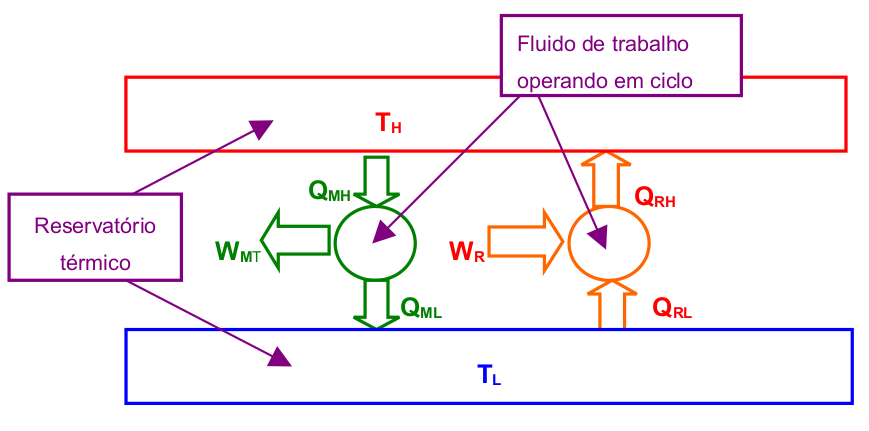
\includegraphics[
            width=0.85\textwidth
        ]   {cyclicMachinesSecondLaw.tex}

        \label{fig:cyclicMachinesSecondLaw}
    \end{figure}

    Refrigeradores e bombas de calor (\cref{fig:cyclicMachinesSecondLaw}), por
    sua vez, são sistemas termodinâmicos fechados cujo fluido de trabalho opera
    em processo cíclico, e que produzem a transferência de calor de um corpo a
    temperatura mais baixa a outro a temperatura mais elevada, às custas de
    trabalho líquido ou de calor.

    Refrigeradores propriamente ditos são aqueles em que a fonte quente (que
    recebe calor) é o meio-ambiente a \gsub{temperature}{environmentState}.
    Assim, o papel de um refrigerador é, através da carga térmica de uma fonte
    fria, manter frio um espaço frio (pense em sua geladeira doméstica).

    Bombas de calor, por outro lado, são aquelas máquinas em que a fonte fria
    (que emite o calor) é o meio-ambiente a
    \gsub{temperature}{environmentState}. Assim, o papel de uma bomba de calor
    é, através da carga térmica de uma fonte quente, manter quente um espaço
    quente (pense em um meio-ambiente a \SI{-10}{\celsius} e uma sala que tem
    que se manter a \SI{21}{\celsius}).

    A variação de entropia dos ciclos da máquina térmica (\gls{cyclicMachine})
    e do refrigerador (\gls{refrigerator}) é zero, de tal forma que o
    inventário de entropia envolve apenas e tão somente os reservatórios
    térmicos \gsub{temperature}{hotReservoir} e
    \gsub{temperature}{coldReservoir}. Da mesma forma, a variação da energia
    interna dos ciclos é zero, de modo que o balanço de energia envolve os
    calores $\gls{heatTransfer}_{\gls{cyclicMachine}\gls{hotReservoir}}$,
    $\gls{heatTransfer}_{\gls{cyclicMachine}\gls{coldReservoir}}$,
    $\gls{heatTransfer}_{\gls{refrigerator}\gls{hotReservoir}}$ e
    $\gls{heatTransfer}_{\gls{refrigerator}\gls{coldReservoir}}$ trocados entre os
    reservatórios e os ciclos, bem como os respectivos trabalhos
    \gsub{workTransfer}{cyclicMachine} e \gsub{heatTransfer}{refrigerator}.
    Quando se discute máquinas térmicas, costuma-se adotar as grandezas em
    módulo de tal forma que o sinal será dado pela própria formulação. Assim
    %
    \begin{equation} \label{eq:3.10}
        \gsub{workTransfer}{cyclicMachine}
        =
        \gls{heatTransfer}_{\gls{cyclicMachine}\gls{hotReservoir}}
        -
        \gls{heatTransfer}_{\gls{cyclicMachine}\gls{coldReservoir}}
        \,\,\,\,
        %
        \text{e}
        %
        \,\,\,\,
        \gls{heatTransfer}_{\gls{refrigerator}\gls{coldReservoir}}
        =
        \gls{heatTransfer}_{\gls{cyclicMachine}\gls{hotReservoir}}
        -
        \gsub{workTransfer}{refrigerator}\,,
    \end{equation}
    %
    \begin{equation} \label{eq:3.11}
        \frac{
            \gls{heatTransfer}_{\gls{cyclicMachine}\gls{hotReservoir}}
        }{
            \gsub{temperature}{hotReservoir}
        }
        -
        \frac{
            \gls{heatTransfer}_{\gls{cyclicMachine}\gls{coldReservoir}}
        }{
            \gsub{temperature}{coldReservoir}
        }
        \le 0
        \,\,\,\,
        %
        \text{e}
        %
        \,\,\,\,
        \frac{
            \gls{heatTransfer}_{\gls{refrigerator}\gls{coldReservoir}}
        }{
            \gsub{temperature}{coldReservoir}
        }
        -
        \frac{
            \gls{heatTransfer}_{\gls{refrigerator}\gls{hotReservoir}}
        }{
            \gsub{temperature}{hotReservoir}
        }
        \le 0\,.
    \end{equation}

    Vamos definir o rendimento da máquina térmica como sendo a razão entre a
    energia que se deseja e a energia que se gasta. Assim:
    %
    \begin{equation} \label{eq:efficiencyOfCyclicMachine}
        \gsub{efficiency}{cyclicMachine}
        =
        \frac{
            \gsub{workTransfer}{cyclicMachine}
        }{
            \gls{heatTransfer}_{\gls{cyclicMachine}\gls{hotReservoir}}
        }
        =
        1
        -
        \frac{
            \gls{heatTransfer}_{\gls{cyclicMachine}\gls{coldReservoir}}
        }{
            \gls{heatTransfer}_{\gls{cyclicMachine}\gls{hotReservoir}}
        }\,.
    \end{equation}

    Vamos definir o coeficiente de performance de um refrigerador como a razão
    entre a carga térmica, isto é, a energia retirada da fonte fria, sobre a
    energia gasta para isso, na forma de trabalho mecânico ou calor.
    Consideremos o caso comum de trabalho mecânico. Da mesma forma, definimos o
    coeficiente de performance da bomba de calor. Então:
    %
    \begin{equation} \label{eq:performanceCoefficient}
        \gsub{performanceCoeff}{refrigerator}
        =
        \frac{
            \gls{heatTransfer}_{\gls{refrigerator}\gls{coldReservoir}}
        }{
            \gsub{workTransfer}{refrigerator}
        }
        \,\,\,\,
        %
        \text{e}
        %
        \,\,\,\,
        \gsub{performanceCoeff}{heatPump}
        =
        \frac{
            \gls{heatTransfer}_{\gls{refrigerator}\gls{hotReservoir}}
        }{
            \gsub{workTransfer}{refrigerator}
        }\,.
    \end{equation}

    Se o ciclo for \emph{completamente reversível (interna e externamente)} é
    denominado \emph{Ciclo de Carnot}. Você pode então demonstrar que:

    \begin{enumerate}
        \item o rendimento do Ciclo de Carnot não depende do fluido de trabalho
            do ciclo e pode ser expresso apenas em termos das temperaturas
            \gsub{temperature}{coldReservoir} e
            \gsub{temperature}{hotReservoir}, da seguinte forma:
            %
            \begin{equation} \label{eq:efficiencyOfCarnotCycle}
                \gsub{efficiency}{CarnotCycle}
                =
                1
                -
                \frac{
                    \gsub{temperature}{coldReservoir}
                }{
                    \gsub{temperature}{hotReservoir}
                }
            \end{equation}

        \item não existe rendimento de máquina térmica, reversível ou não,
            maior do que o de Carnot quando operando entre os mesmos
            reservatórios térmicos e que

        \item o rendimento do Ciclo de Carnot é sempre menor do que
            \SI{100}{\percent}.
    \end{enumerate}

    Analise o enunciado de Kelvin-Planck da Segunda Lei:
    \emph{%
        É impossível construir um dispositivo que opere num ciclo e que não
        produza outros efeitos além da realização de trabalho e da troca de
        calor com um único reservatório térmico.%
    }

    Então compare com o enunciado proposto por Clausius:
    \emph{%
        É impossível realizar um dispositivo que opere em um ciclo e que não
        produza outros efeitos que a passagem de calor de um corpo frio para
        outro mais quente.%
    }

    Pois bem, utilizando a nossa formulação da Segunda Lei, agora você deve ser
    capaz de demonstrar a equivalência de todos estes enunciados.

    Finalmente, lembre-se que, assim como a Primeira Lei, você não pode provar
    ou disprovar as Leis da Termodinâmica, elas são postuladas...


    \section{A Segunda Lei para Sistema Aberto}

    Existem claramente três maneiras de se alterar a entropia no interior de um
    sistema aberto durante o intervalo de tempo \diff{\gls{time}}:

    A primeira, através dos fluxos de calor \idiff{\gls{heatTransfer}_{j}},
    provenientes de fontes a \state{\gls{temperature}}{j} que atravessam as
    regiões da superfície de controle cuja temperatura local é
    \state{\gls{temperature}}{j}, por meio da avaliação dos
    $\dfrac{\idiff{\gls{heatTransfer}_{j}}}{\state{\gls{temperature}}{j}}$;

    A segunda, através do fluxo líquido de entropia que atravessa a superfície
    de controle transportada pelas massas \idiff{\gsub{mass}{inlet}},
    \idiff{\gsub{mass}{outlet}};

    E a terceira, por meio da produção irreversível de entropia
    \idiff{\gls{entropyCreated}}, que leva em conta todas as
    irreversibilidades.

    Se separarmos, por conveniência futura, o calor
    \idiff{\gsub{heatTransfer}{environmentState}} proveniente do reservatório
    do meio-ambiente a \gsub{temperature}{environmentState}, podemos expressar,
    sinteticamente:
    %
    \begin{equation} \label{eq:3.12}
        \diff{\gsub{entropy}{controlVolume}}
        =
        \diff
        \left(
            \gls{mass}
            \gls{entropy}
        \right)_{\gls{controlVolume}}
        =
        \underset{\gls{inlet}}{\sum }{
            \idiff{\gsub{mass}{inlet}}
            \gsub{intEntropy}{inlet}
        }
        -
        \underset{\gls{outlet}}{\sum }{
            \idiff{\gsub{mass}{outlet}}
            \gsub{intEntropy}{outlet}
        }
        +
        \underset{j \neq \gls{environmentState}}{\sum }{
            \frac{
                \idiff{\gls{heatTransfer}_{j}}
            }{
                \state{\gls{temperature}}{j}
            }
        }
        +
        \frac{
            \idiff{\gsub{heatTransfer}{environmentState}}
        }{
            \gsub{temperature}{environmentState}
        }
        +
        \idiff{\gls{entropyCreated}}\,,
        \,\,\,\,
        \idiff{\gls{entropyCreated}} \ge 0\,,
    \end{equation}
    %
    ou, na forma de equação diferencial:
    %
    \begin{equation} \label{eq:3.13}
        \DDt{\gsub{entropy}{controlVolume}}
        =
        \DDt{}
        \left(
            \gls{mass}
            \gls{entropy}
        \right)_{\gls{controlVolume}}
        =
        \underset{\gls{inlet}}{\sum }{
            \gsub{massFlowRate}{inlet}
            \gsub{intEntropy}{inlet}
        }
        -
        \underset{\gls{outlet}}{\sum }{
            \gsub{massFlowRate}{outlet}
            \gsub{intEntropy}{outlet}
        }
        +
        \underset{j \neq \gls{environmentState}}{\sum }{
            \frac{
                \gls{heatTransferRate}_{j}
            }{
                \state{\gls{temperature}}{j}
            }
        }
        +
        \frac{
            \gsub{heatTransferRate}{environmentState}
        }{
            \gsub{temperature}{environmentState}
        }
        +
        \gls{entropyCreatedRate}\,,
        \,\,\,\,
        \gls{entropyCreatedRate} \ge 0\,.
    \end{equation}

    Integrando-se a \cref{eq:3.12} ou \ref{eq:3.13} no processo especificado
    $A$ que leva do estado 1 ao estado 2, obtemos
    %
    \begin{equation} \label{eq:3.14}
        \begin{aligned}
        \left(
            \state{\gls{mass}}{2}
            \state{\gls{intEntropy}}{2}
            -
            \state{\gls{mass}}{1}
            \state{\gls{intEntropy}}{1}
        \right)_{\gls{controlVolume}}
        &=
        \underset{\gls{inlet}}{\sum }{
            \int\limits_1^2{
                \gsub{intEntropy}{inlet}
            }\idiff\gsub{mass}{inlet}
        }
        -
        \underset{\gls{outlet}}{\sum }{
            \int\limits_1^2{
                \gsub{intEntropy}{outlet}
            }\idiff\gsub{mass}{outlet}
        }
        +\\
        %
        &+
        \underset{j \neq \gls{environmentState}}{\sum }{
            \int\limits_1^2
            \frac{
                \gls{heatTransferRate}_{j}
            }{
                \state{\gls{temperature}}{j}
            }\bigg)_A
        }
        +
        \frac{
            \fprocess{heatTransfer}{1}{2\gls{environmentState}}{A}
        }{
            \gsub{temperature}{environmentState}
        }
        +
        \fprocess{entropyCreated}{1}{2}{A}\,,
        \end{aligned}
    \end{equation}
    %
    e para que as integrais possam ser avaliadas, precisamos conhecer as
    respectivas funções para $\gsub{intEntropy}{inlet},
    \gsub{intEntropy}{outlet}, \idiff{\gls{heatTransfer}_j},
    \state{\gls{temperature}}{j}, j \neq 0$ ao longo do processo particular $A$ que
    vai do estado 1 para o estado 2. Uma vez que
    \gsub{temperature}{environmentState} é constante, podemos expressar o calor
    total trocado com o meio-ambiente, que varia com o processo, por
    \fprocess{heatTransfer}{1}{2\gls{environmentState}}{A}.


    \section{O Regime Permanente}

    Eliminando-se a dependência explícita no tempo, ou seja, assumindo que
    todos os termos são constantes, obtemos novamente uma equação algébrica:
    %
    \begin{equation} \label{eq:3.15}
        \gls{entropyCreatedRate}
        =
        \underset{\gls{inlet}}{\sum }{
            \gsub{massFlowRate}{inlet}
            \gsub{intEntropy}{inlet}
        }
        -
        \underset{\gls{outlet}}{\sum }{
            \gsub{massFlowRate}{outlet}
            \gsub{intEntropy}{outlet}
        }
        +
        \underset{j \neq \gls{environmentState}}{\sum }{
            \frac{
                \gls{heatTransferRate}_{j}
            }{
                \state{\gls{temperature}}{j}
            }
        }
        +
        \frac{
            \gsub{heatTransferRate}{environmentState}
        }{
            \gsub{temperature}{environmentState}
        }\,,
        \,\,\,\,
        \gls{entropyCreatedRate} \ge 0\,.
    \end{equation}

    Seja um processo adiabático e em regime permanente que ocorre em um volume
    de controle com uma única entrada e uma única saída de massa (você consegue
    imaginar uma aplicação deste modelo?). Então, utilizando a conservação de
    massa, concluímos pela Segunda Lei que
    %
    \begin{equation} \label{eq:3.16}
        \gsub{intEntropy}{outet}
        \ge
        \gsub{intEntropy}{inlet}\,,
    \end{equation}
    %
    e, pela Primeira Lei:
    %
    \begin{equation} \label{eq:3.17}
        \gls{specifcWorkRate}
        =
        \frac{
            \gsub{workTransferRate}{controlvolume}
        }{
            \gls{massFlowRate}
        }
        =
        \gsub{intEntropy}{inlet}
        -
        \gsub{intEntropy}{inlet}\,.
    \end{equation}


    \section{Regime Transiente}

    Se existe a dependência com o tempo, então trata-se do regime transiente.
    Nesse caso, cada problema deve ser analisado cuidadosamente, frequentemente
    a partir das equações na forma de diferenciais, como no exemplo a seguir.

    Seja um tanque rígido cheio de gás em um estado definido. A partir de um
    determinado instante, passa a ocorrer um vazamento rápido, através de um
    processo de descompressão que pode ser considerado adiabático. Investigue o
    modelamento do vazamento. Se o vazamento for para o meio-ambiente a
    \gsub{temperature}{environmentState}, \gsub{pressure}{environmentState},
    até quando ele ocorrerá?

    Trata-se claramente de um processo transiente com apenas uma saída de
    massa. Pela Primeira Lei para sistema aberto, assumindo processo adiabático
    e fronteira rígida, desprezando as energias cinéticas e potenciais,
    simplificamos a \cref{eq:2.15} na forma diferencial para obtermos:
    %
    \begin{equation} \label{eq:3.18}
        \diff{(
            \gls{mass}
            \gls{intInternalEnergy}
        )}_{\gls{controlVolume}}
        =
        -\gsub{intEnthalpy}{outlet}
        \idiff{\gsub{mass}{outlet}}\,.
    \end{equation}

    Pela Segunda Lei, simplificando-se a Eq. 3.12:
    %
    \begin{equation} \label{eq:3.19}
        \diff{(
            \gls{mass}
            \gls{intEntropy}
        )}_{\gls{controlVolume}}
        =
        -\gsub{intEntropy}{outlet}
        \idiff{\gsub{mass}{outlet}}
        +
        \idiff{\gls{entropyCreated}}\,,
        \,\,\,\,
        \idiff{\gls{entropyCreated}} \ge 0\,.
    \end{equation}

    Pela conservação de massa:
    %
    \begin{equation} \label{eq:3.20}
        \diff{\gsub{mass}{controlVolume}}
        =
        -\idiff{\gsub{mass}{outlet}}\,.
    \end{equation}

    Expandindo-se na \cref{eq:3.18,eq:3.19} respectivamente a energia interna e
    a entropia total do volume de controle e substituindo nelas a
    \cref{eq:3.20}:
    %
    \begin{equation} \label{eq:3.21}
        \gsub{intInternalEnergy}{controlVolume}
        \diff{\gsub{mass}{controlVolume}}
        +
        \gsub{mass}{controlVolume}
        \diff{\gsub{intInternalEnergy}{controlVolume}}
        =
        \gsub{intEnthalpy}{outlet}
        \diff{\gsub{mass}{controlVolume}}
        =
        \gsub{intInternalEnergy}{outlet}
        \diff{\gsub{mass}{controlVolume}}
        +
        (\gls{pressure}\gls{specificVolume})_{\gls{outlet}}
        \diff{\gsub{mass}{controlVolume}}\,,
    \end{equation}
    %
    \begin{equation} \label{eq:3.22}
        \gsub{intEntropy}{controlVolume}
        \diff{\gsub{mass}{controlVolume}}
        +
        \gsub{mass}{controlVolume}
        \diff{\gsub{intEntropy}{controlVolume}}
        =
        \gsub{intEntropy}{outlet}
        \diff{\gsub{mass}{controlVolume}}
        +
        \idiff{\gls{entropyCreated}}\,,
        \,\,\,\,
        \idiff{\gls{entropyCreated}} \ge 0\,.
    \end{equation}

    Consideremos agora que o estado de saída seja o estado instantâneo do
    interior do volume de controle. Então
    $\gsub{intInternalEnergy}{controlVolume} =
    \gsub{intInternalEnergy}{outlet}$ e
    $(\gls{pressure}\gls{specificVolume})_{\gls{controlVolume}} =
    (\gls{pressure}\gls{specificVolume})_{\gls{outlet}}$. Além disso,
    %
    \begin{equation}
        \diff{(
            \gls{mass}
            \gls{specificVolume}
        )}_{\gls{controlVolume}}
        =
        \gsub{mass}{controlVolume}
        \diff{
            \gls{specificVolume}
        }_{\gls{controlVolume}}
        +
        \gsub{specificVolume}{controlVolume}
        \diff{
            \gls{mass}
        }_{\gls{controlVolume}}\,,
    \end{equation}
    %
    e, portanto,
    %
    \begin{equation} \label{eq:3.23}
        \gsub{mass}{controlVolume}
        \diff{\gsub{intInternalEnergy}{controlVolume}}
        =
        (\gls{pressure}\gls{specificVolume})_{\gls{controlVolume}}
        \diff{\gsub{mass}{controlVolume}}
        =
        -\gsub{mass}{controlVolume}
        \gsub{pressure}{controlVolume}
        \diff{\gsub{specificVolume}{controlVolume}}\,,
    \end{equation}
    %
    de onde obtemos que
    %
    \begin{equation} \label{eq:3.24}
        \left(
            \diff{\gls{intInternalEnergy}}
            +
            \gls{pressure}
            \diff{\gls{specificVolume}}
        \right)_{\gls{controlVolume}}
        =
        0\,.
    \end{equation}

    O resultado na \cref{eq:3.24} tem importantes implicações que só poderão
    ser discutidas posteriormente, quando estudarmos as relações entre as
    propriedades termodinâmicas. Por outro lado,
    %
    \begin{equation} \label{eq:3.25}
        \gsub{intEntropy}{controlVolume}
        \approx
        \gsub{intEntropy}{outlet}\,,
    \end{equation}
    %
    pois a entropia da massa que sai pode ser considerada igual à da massa que
    resta no volume de controle, se desprezarmos o processo irreversível no
    local do vazamento. Assim,
    %
    \begin{equation} \label{eq:3.26}
        \gsub{mass}{controlVolume}
        \diff{\gsub{intEntropy}{controlVolume}}
        \approx
        \idiff{\gls{entropyCreated}}
        \ge 0\,,
    \end{equation}
    %
    se levarmos em conta as irreversibilidades internas no processo de
    esvaziamento. Agora, se considerarmos o processo como reversível,
    %
    \begin{equation}
        \diff{\gsub{intEntropy}{controlVolume}}
        =
        0
    \end{equation}
    %
    ou
    %
    \begin{equation} \label{eq:3.27}
        \gsub{intEntropy}{controlVolume}
        =
        constante\,,
    \end{equation}
    %
    ou seja, o vazamento adiabático poderia ser modelado como se a entropia
    específica da massa restante no tanque não se alterasse, ou em outros
    termos, a massa restante sofreria um processo adiabático reversível, um
    resultado curioso, mas bastante utilizado na prática.

    Agora refaça o problema do esvaziamento do tanque, só que considere o
    esvaziamento tão lento que ocorre isotermicamente, ou seja, o sistema troca
    calor com o meio-ambiente durante todo o processo. Você consegue imaginar
    algum exemplo real desse processo? Perceba que os processos reais de
    vazamento geralmente ocorrerão entre estas duas hipóteses: adiabático e
    isotérmico.
